\chapter{دسته‌بندی حیوانات با استفاده از یادگیری بدون نمونه}
\label{chap:one}
در ادامه توضیحات ارائه شده در پیش‌گفتار  و فصل پیشین درباره یادگیری بدون نمونه، در رابطه با دسته‌بندی حیوانات مقاله 
\cite{Lampert2014} 
را مورد بررسی قرار داده‌ایم. این مقاله با یادگیری مشخصه‌هایی موسوم به ویژگی‌های  
\trans{معنایی}{Semantic}
یا ویژگی‌های سطح بالا سعی در دسته‌بندی حیوانات دارد؛ به طور مثال: آبزی یا خشک‌زی بودن، گیاه خوار یا گوشت خوار بودن، راه راه یا خال خال یا ساده بودن، اندازه جثه، رنگ پوست و صفاتی از این قبیل، صفات معنایی نامیده می‌شوند. 

مشخصه‌هایی که انسان با استفاده از آن‌ها می‌تواند بدون پیش‌زمینه‌ای با مشاهده اولین نوع از یک چیز آن را دسته‌بندی کند. فرض کنید که مدل، اسب و ببر را دیده و دسته‌بندی کرده‌است حالا باید بتواند گورخر را که تا کنون نمونه‌ای از آن را ندیده است و جثه‌ای مشابه اسب و طرح پوستی شبیه به ببر را دارد بدون نیاز به اطلاعات بیشتری و با استفاده از اطلاعات قبلی در یک دسته‌بندی جدید قرار دهد. به همین دلیل به ویژگی‌های معنایی نیاز پیدا می‌کنیم.
\section{مدل یادگیری}
مقاله مطالعه شده روشی برای دسته بندی بر اساس ویژگی‌های معنایی به همراه یک پایگاه داده مرتبط ارائه کرده است
 \cite{Lampert2014}.
پایگاه داده ارائه شده شامل بیش از ۳۰۰۰۰ تصویر حیوانات در ۵۰ دسته مختلف و ۸۵ ویژگی معنایی است. انسان قادر است تا حدود ۳۰۰۰۰ دسته پایه از جیز‌های مختلف را تشخیص دهد. هدف بینایی ماشین همواره نزدیک کردن ماشین به انسان بوده است. 
 
در شکل
\ref{fig:sample}
نحوه دسته بندی حیوانات مختلف توسط روش ارائه شده را می‌توان مشاهده کرد. ویژگی‌های معنایی که ارتباط، شباهت و یا تفاوت های موجودات را بیان می‌کنند برای دسته‌بندی استفاده شده‌اند.
%\newpage
\begin{figure}
	\centering
	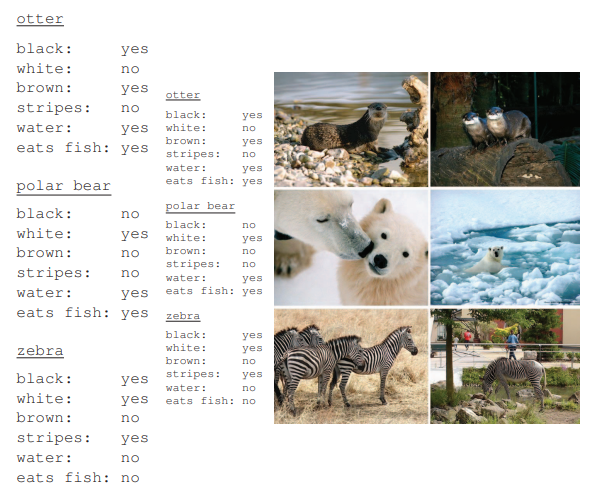
\includegraphics[width=0.8\textwidth]{img/report/sample}
	\caption{نحوه دسته بندی تصاویر توسط مدل ارائه شده \cite{Lampert2014}}
	\label{fig:sample}
	\centering
\end{figure}

مقاله از سه روش برای دسته‌بندی نام برده‌است و آن‌ها را با یکدیگر مقایسه می‌کند.	
\trans{دسته بندی چندکلاسه مسطح}{flat multi-class classification}،
\trans{پیش بینی مشخصه به طور مستقیم}{direct attribute prediction} و 
\trans{پیش بینی مشخصه به طور غیر مستقیم }{indirect attribute prediction}
به طور شهودی این سه روش در شکل 
\ref{fig:learning-methods}
نشان داده شده‌اند.
به دلیل این‌که همواره نمی‌توان پایگاه داده‌ای کامل و برچسب خورده داشت نیازمند راهکار‌هایی هستیم تا تلاش انسان در جمع‌آوری و دسته‌بندی‌ داده‌ها را کم کنیم.

در شکل
\ref{fig:learning-methods}
تصویر الف، نشان دهنده روش اول است. در این روش ماشین یک بردار ثابت را یاد میگیرد. x ورودی مسئله، y برچسب‌ داده‌ها آزمایش و z برچسب داده‌هایی است که نیاز داریم آن‌ها را بیابیم. چون فرآيند یادگیری y هیچ تاثیری بر فرآیند یادگیری z ندارد پس از یادگیری‌های قبلی برای پیش بینی نمی‌توان استفاده کرد و این روش یک روش یادگیری معمولی است که قبلا نیز استفاده می‌شد و برای یادگیری z نیازمند داده‌های ورودی هستیم که با توجه به اینکه به دنبال یادگیری بدون نمونه هستیم این روش مناسب نیست.

راهکار ارائه شده برای یادگیری استفاده از ویژگی‌های معنایی سطح بالایی هستند که هرکدام برای انسان معنای خاصی دارند. این مشخصه‌ها، ویژگی‌های قابل نام‌گذاری هستند؛ مانند: رنگ، شکل، طرح بدن و عادات غذایی. استفاده از این مشخصه‌‌ها به ما کمک می‌کند تا نقش انسان را در فرآیند یادگیری کمتر کنیم و نیاز کمتری به ویژگی‌های سطح پایین تصویر داشته باشیم.

\begin{figure}[b]
	
	\centering
	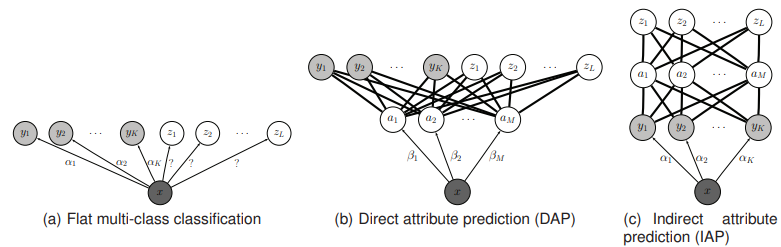
\includegraphics[width=\textwidth]{img/report/learning-methods}
	\caption{روش‌های دسته‌بندی \cite{Lampert2014}}
	\label{fig:learning-methods}
	\centering
\end{figure}

\newpage
این مشخصه‌ها را می‌توان همراه با تصاویر یا همراه با دسته‌بندی‌های تصاویر درنظر گرفت و این ویژگی باعث شده است تا فرآیند 
\trans{دسته‌بندی بر اساس مشخصه‌ها}{attribute-based classification}
توسط مقاله معرفی شود. در این فرآیند با توجه به اینکه دسته‌های آموزش و آزمایش جدا از هم هستند و به یکدیگر وابسته نیستند؛ می‌توان با استفاده از این صفات و 
\trans{انتقال یادگیری}{transfer learning}،
 بین داده‌های آموزشی، داده‌های آزمایشی را دسته‌بندی کرد. در شکل 
\ref{fig:sample}
می‌توانید نحوه دسته‌بندی بر اساس صفات را مشاهده کنید.
با توجه به توضیحات ارائه شده به سراغ توضیح دو روش دیگر می‌رویم.
\subsection{روش مستقیم}
در روش 
\trans{پیش‌بینی مشخصه‌ به صورت مستقیم}{direct attribute prediction}
یا DAP در مرحله آموزش کلاس خروجی هر نمونه (x) برای لایه مشخصه‌ها نیز به طور قطع یک برچسب (y) مشخص می‌کند. متعاقبا می‌توان از هر روش با نظارتی استفاده کرد و  پارامتر‌های هر مشخصه‌ 
\textsubscript{m}$\beta$ 
را پیدا کرد. این بدین معنی است که فرآیند یادگیری اولیه برای یادگیری مشخصه‌ها متناسب با هر نمونه و دسته‌بندی مشخصه‌ها و نمونه‌ها را می‌توان با یک روش یادگیری نظارتی ساده انجام داد. حال با استفاده از یادگیری انتقالی و استفاده از شبکه‌ای که از پیش نمونه‌ها و مشخصه‌ها آن دسته‌بندی شده‌اند برای نمونه‌های جدید   که از پیش دیده نشده‌اند (داده‌های آزمون) دسته‌بندی جدیدی را فقط بر اساس لایه مشخصه‌ها وزن‌ها یا پارامتر‌هایی که شبکه تا به حال دارد و به لایه مشخصه‌ها اختصاص داده‌است، استفاده کرد و داده جدید را دسته‌بندی کرد.

\subsection{روش غیر مستقیم}
در روش 
\trans{پیش‌بینی مشخصه‌ به صورت غیر مستقیم}{indirect attribute prediction}
یا IAP همانند روش قبل از مشخصه‌ها برای انتقال دانش بین دسته‌ها استفاده می‌کند اما اینبار مشخصه‌ها بین دولایه از برچسب‌ها قرار دارند. یک لایه برچسب‌هایی که در لایه آموزش اختصاص می‌یابند (y) و یک لایه برچسب‌هایی که باید به داده‌های جدید اختصاص پیدا کنند (z) . در مرحله آموزش پارامتر‌های لایه مشخصه‌ها توسط برچسب‌های آموزش مقدار دهی می‌شوند همانند یک مسئله دسته‌بندی چند‌کلاسه که می‌توان با یک روش نظارتی ساده نیز یادگیری را انجام داد. در مرحله آزمایش با استفاده از مقادیری که به لایه مشخصه‌ها اختصاص داده‌شده دسته‌بندی داده‌های آزمایش را صورت می‌گیرد. استفاده از لایه مشخصه‌ها به برای دسته‌بندی داده‌های آزمایش این امکان را می‌دهد تا بتوانیم عملیاتی مشابه 
\trans{تنظیم}{regularization}
را انجام دهیم و فقط ترکیبات با معنی از مشخصه‌ها را ایجاد کنیم.

روش‌های یاد شده یک سری استراتژی کلی محسوب می‌شوند که می‌توانند با ترکیبی از روش‌‌های موجود مانند: یادگیری با نظارت یا رگرسیون‌ها  بر روی مشخصه‌ها تصاویر یا دسته‌های تصاویر با استفاده از پارامتر‌های پیش‌بینی شده انجام شوند. در این مقاله از روش توزیع‌های احتمالاتی استفاده شده و مشخصه‌های استفاده شده را مشخصه‌هایی بله یا خیر در نظر گرفته‌است. برای مشخصه‌هایی که بله یا خیر نیستند می‌توان به جای دسته‌بندی از رگرسیون استفاده کرد.

در روش DAP برای دسته‌بندی کردن تصاویر آزمون، احتمال قطعی به دست خواهد آمد زیرا در مرحله آموزش لایه مشخصه‌ها مقادیر مناسب را اتخاذ می‌کنند و از همین مقادیر برای تصاویر آزمون نیز استفاده می‌شود. به زبان ریاضی معادلات زیر صادق است.


\begin{equation}
	p(z|x) = \sum_{a\in(0,1)^{M}} p(z|a)p(a|x)\dfrac{p(z)}{p(a^{a})}\prod_{m=1}^{M} p(a_{m}^{z}|x).
\end{equation}

\begin{equation}
f(x) = \argmax\limits_{l=1,...,L} p(z=l|x) = \argmax\limits_{l=1,...,L} \prod_{m=1}^{M} \dfrac{p(a_{m}^{z_{l}}|x)}{p(a_{m}^{z_{l}})}.
\label{eq:2}
\end{equation}

در روش IAP لایه مشخصه‌ها نقش یک تنظیم‌کننده را ایفا می‌کند پس به طور قطع نمی‌توان برای تشخیص لایه آزمون استفاده کرد و می‌بایست با استفاده از روابط احتمال یک احتمال میانی را حساب کرد و پس از آن از رابطه
\ref{eq:2}
استفاده کرد.
\begin{equation}
p(a_{m}|x) = \sum_{k=1}^{K} p(a_{m}|y_{k})p(y_{k}|x).
\end{equation}


\subsection{بانک‌های اطلاعاتی}
سه بانک اطلاعاتی استفاده شده است. در ادامه هر یک را توضیح می‌دهیم.
\ref{table:Datasets}
\subsubsection{\lr{Animal with Attributes}}

این بانک اطلاعاتی به عنوان بانک اصلی استفاده شده است. این بانک شامل ۵۰ کلاس حیوانات و ۸۵ کلاس مشخصه‌های معنایی است؛ از این تعداد ۴۰ کلاس به عنوان داده‌های آموزشی و ۱۰ کلاس به عنوان داده‌های آزمایش استفاده شده است. تقسیم بندی به صورت تصادفی نیست اما سعی شده است تا توزیع داده‌ها در هر دو دسته آزمایش و آزمون به طور مناسبی صورت شود.

در کل 30475 عکس در این بانک داده وجود دارد که تعداد تصاویر برای دسته‌های مختلف حیوانات متفاوت می‌باشد. برای تسریع در محاسبات یک سری از ویژگی‌های تصاویر مانند: جنبه‌های رنگ، بافت و شکل، هیستوگرام رنگ و سایر ویژگی‌های مهم تصویر نیز به پایگاه داده اضافه شده‌و برای آموزش از روش 
\lr{5 fold cross-validation}
استفاده شده‌است.

\subsubsection{\lr{aPascal-aYahoo}}

این بانک شامل دو دسته داده یکی داده‌های بانک داده PASCAL و دیگری داده‌هایی که از موتور جستجوی Yahoo استخراج شده است. ۲۰ کلاس داده در PASCAL و ۱۲ کلاس داده در Yahoo و دسته‌بندی داده‌ها در هر یک با دیگری متفاوت است پس می‌توان از داده‌های PASCAL برای آموزش و از داده‌های Yahoo برای آزمون استفاده کرد. هر تصویر ۶۴ مشخصه‌ها دودویی را شامل ‌می‌شود و همانند بانک داده قبلی برای تسریع در محاسبات یک سری از ویژگی‌های تصاویر از قبل محاسبه شده‌اند.

\subsubsection{\lr{SUN Attributes}}

این بانک زیر مجموعه‌ای از بانک داده‌
\lr{SUN Database}
که شامل 717 کلاس داده و هر تصویر شامل ۱۰۲ مشخصه‌ دودویی است. این مشخصه‌ها شامل توضیفات صحنه، شرایط نورپردازی، مواد داخل تصویر و ... است.

\begin{table}[h]
	\begin{center}
	\begin{tabular}{c|c|c|c} 
		Dataset & AwA & aP/aY & SUN \\
		\hline \lr{\# Images} & 30475 & 15339 & 14340 \\
		\lr{\# Classes} & 50 & 32 & 717 \\
		\lr{\# Attributes} & 85 & 64 & 102 \\
		\lr{Annotation Level} & per class & per image & per image \\
		Annotation Type (real- & both & binary & binary \\
		valued or binary) & &
	\end{tabular}
	\caption{بانک‌های اطلاعاتی \cite{Lampert2014}}
	\label{table:Datasets}
	\end{center}
\end{table}
%\begin{figure}[h]
%	\centering
%	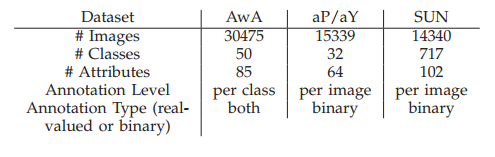
\includegraphics[width=0.6\textwidth]{img/report/Datasets}
%	\caption{بانک‌های اطلاعاتی \cite{Lampert2014}}
%	\label{fig:Datasets}
%	\centering
%\end{figure}

\subsection{ارزیابی}

برای این کار از 
\trans{ماشین بردار پشتیبان}{Support Vector Machine} یا SVM
استفاده شده‌‌است. برای روش مستقیم از یک SVM غیر خطی و برای روش غیرمستقیم از نوع
\lr{one-versus-rest}
استفاده شده‌است.
نتایج به دست آمده را در جداول 
\ref{table:result1}
\ref{table:result2}
مشاهده می‌کنید.


\begin{table}[h]
	\begin{center}
\begin{tabular}{c|cc|cc|c} 
	method & DAP & IAP & CT-cc & CT-H & rnd \\
	\hline \lr{MC acc.} & 41.4 & 42.2 & $30.7 \pm 0.2$ & $30.8 \pm 0.2$ & 10.0 \\
	classAUC & 81.4 & 80.0 & 73.4 & 73.4 & 50.0 \\
	attrAUC & 72.8 & 72.1 & $-$ & $-$ & 50.0
\end{tabular}
	\caption{تقسیم بندی پیش‌فرض داده‌ها \cite{Lampert2014}}
	\label{table:result1}
	\end{center}
\end{table}
\begin{table}[h]
	\begin{center}
	 \begin{tabular}{c|cc|cc|c} 
	method & DAP & LAP & CT-cc & CT-H & md \\
	\hline \lr{MC acc.} & $37.1 \pm 3.9$ & $34.1 \pm 5.1$ & $27.7 \pm 4.3$ & $27.3 \pm 4.0$ & 10.0 \\
	classAUC & $80.4 \pm 3.1$ & $76.3 \pm 5.5$ & $72.4 \pm 2.7$ & $72.8 \pm 3.1$ & 50.0 \\
	attrAUC & $70.7 \pm 3.5$ & $69.7 \pm 3.8$ & $-$ & $-$ & 50.0
\end{tabular}
	\caption{تقسیم بندی داده‌ها به صورت تصادفی \cite{Lampert2014}}
	\label{table:result2}
	\end{center}
\end{table}

%\begin{figure}[b]
%	\centering
%	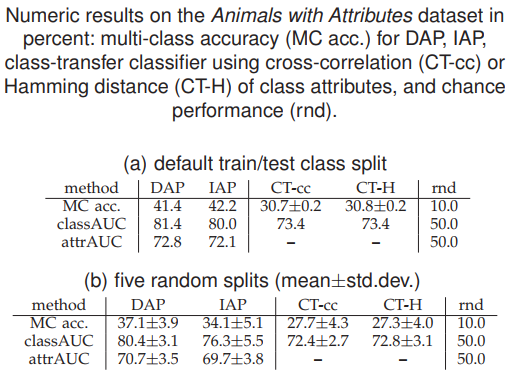
\includegraphics[width=0.5\textwidth]{img/report/results}
%	\caption{نتایج \cite{Lampert2014}}
%	\label{fig:results}
%	\centering
%\end{figure}
در روش مستقیم برای بدست آوردن مقادیر مناسب کرنل SVMاز منحنی
\trans{ROC}{Receiver Operation Characteristic}
و 
\trans{میانگین سطح زیر منحنی}{AUC}
برای صفات و روش
\lr{5 fold cross-validation}
استفاده شده‌است. 

منحنی یاد شده، یک نمودار برای نمایش توانایی ارزیابی یک سیستم دسته‌بندی دودویی محسوب می‌شود که آستانه تشخیص آن نیز متغیر است. که با ترسیم نسبت 
\trans{نرخ مثبت صحیح}{True Positive Rate}
 که به اختصار TPR نامیده می‌شود برحسب 
\trans{نرخ مثبت کاذب}{False Positive Rate} 
 با نام اختصاری FPR، ایجاد می‌شود.

در روش غیر مستقیم مراحل مانند روش قبل است با این تفاوت که میانگین سطح زیر منحنی بر روی پیش‌بینی کلاس‌ها استفاده شده‌است.

\begin{figure}[h]
	\centering
	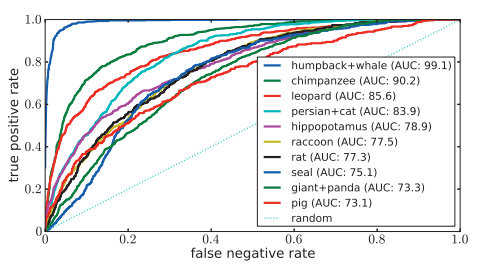
\includegraphics[width=0.6\textwidth]{img/report/ROC}
	\caption{منحنی ROC \cite{Lampert2014}}
	\label{fig:ROC}
	\centering
\end{figure}
همان‌طور که در شکل 
\ref{fig:ROC}
مشاهده می‌کنید. دقت روش در تشخیص برخی از دسته‌ها مانند نهنگ‌های کوهان‌دار دقت بالایی همانند روش‌های یادگیری با نظارت دارد؛ اما در مورد دسته‌بندی‌هایی مانند خوک‌هاو پاندا‌های بزرگ دقت خیلی پایینی دارد. یکی از دلایل این اتفاق شباهت‌هایی است که در این دسته‌ها رخ می‌دهد؛ به طور مثال: ظاهر پاندا‌های بزرگ، خوک‌ها و اسب‌های آبی.

به طور مشابه بر روی دو پایگاه داده دیگر نیز بررسی‌ها انجام شده‌است و نتایج را در جداول 
\ref{table:other_result1}
\ref{table:other_result2}
مشاهده می‌کنید.
%\begin{figure}[h]
%	\centering
%	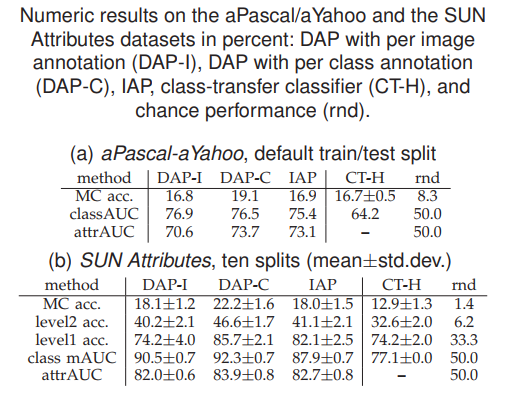
\includegraphics[width=0.5\textwidth]{img/report/other_results}
%	\caption{نتایج بر روی سایر پایگاه‌های داده \cite{Lampert2014}}
%	\label{fig:other_results}
%	\centering
%\end{figure}

\begin{table}[h]
	\begin{center}
	\begin{tabular}{c|ccc|cc} 
	method & DAP-I & DAP-C & IAP & CT-H & rnd \\
	\hline \lr{MC acc.} & 16.8 & 19.1 & 16.9 & $16.7 \pm 0.5$ & 8.3 \\
	classAUC & 76.9 & 76.5 & 75.4 & 64.2 & 50.0 \\
	attrAUC & 70.6 & 73.7 & 73.1 & $-$ & 50.0
	\end{tabular}
	\caption{تقسیم بندی پیش‌فرض داده‌ها برای aPascal-aYahoo \cite{Lampert2014}}
	\label{table::other_result1}
	\end{center}
\end{table}
\begin{table}[h]
	\begin{center}
	 \begin{tabular}{c|ccc|cc} 
	method & DAP-I & DAP-C & IAP & CT-H & rnd \\
	\hline \lr{MC acc.} & $18.1 \pm 1.2$ & $22.2 \pm 1.6$ & $18.0 \pm 1.5$ & $12.9 \pm 1.3$ & 1.4 \\
	\lr{level2 acc.} & $40.2 \pm 2.1$ & $46.6 \pm 1.7$ & $41.1 \pm 2.1$ & $32.6 \pm 2.0$ & 6.2 \\
	\lr{level1 acc.} & $74.2 \pm 4.0$ & $85.7 \pm 2.1$ & $82.1 \pm 2.5$ & $74.2 \pm 2.0$ & 33.3 \\
	\lr{class mAUC} & $90.5 \pm 0.7$ & $92.3 \pm 0.7$ & $87.9 \pm 0.7$ & $77.1 \pm 0.0$ & 50.0 \\
	attrAUC & $82.0 \pm 0.6$ & $83.9 \pm 0.8$ & $82.7 \pm 0.8$ & $-$ & 50.0
\end{tabular}
	\caption{تقسیم بندی داده‌ها برای sub attributes \cite{Lampert2014}}
	\label{table::other_result2}
	\end{center}
\end{table}


\subsection{نتیجه}

هدف این مقاله بدست ‌آوردن درصد‌های بالای دقت دسته‌بندی نبوده است به همین دلیل بسیاری از کار‌های به صورت دستی انجام شده است. هدف اصلی پیاده سازی توانایی انسان در دسته‌بندی بر روی ماشین بوده است؛ که بدین منظور پایگاه‌داده AwA را طراحی کرده‌اند و تلاش کرده‌اند تا بهترین ویژگی‌ها پیدا کنند و این کار یک شروع برای دیگر کار‌ها باشد. همچنین دو روش مستقیم و غیر مستقیم را ارائه کرده که می‌توان با کمی تغییر در آن‌ها برای اهداف مختلف از آن‌‌ها استفاده کرد.
